\documentclass[11pt]{article}

\usepackage{deauthor}
\usepackage{times}
\usepackage{graphicx}
\usepackage{authblk}
\usepackage{hyperref}

\graphicspath{{figs/}}

\title{Plenario: An Open Data Discovery and Exploration Prototype}

\author[1,2]{Charlie Catlett}
\author[2,1]{Brett Goldstein}
\author[2]{Jonathan Giuffrida}
\author[1]{Robert Mitchum}
\author[1]{Alessandro Panella}
\author[3]{Derek Eder}
\author[3]{Eric van Zanten}
\affil[1]{Urban Center for Computation and Data, Computation Institute of the University of Chicago and Argonne National Laboratory}
\affil[2]{Harris School of Public Policy, University of Chicago}
\affil[3]{DataMade, LLC}

%\author{Me}


\begin{document}
\maketitle

\begin{abstract}
The last decade saw a rapid growth in the release of open data by government bodies and public institutions of all sizes. Today hundreds of open data portals, hosting thousands of data sets, represent enormous potential for researchers, policymakers, service providers, journalists, and the general public to better understand the dynamics and processes of cities and ultimately to develop solutions to improve the lives of residents. Given the landscape, a particularly important challenge that has emerged is the sheer lack of capabilities to discover and explore open data to support such processes and inquiries. Plenario is a platform designed to investigate the utility of a system that provides, for users without prior knowledge or expertise in open data, (a) \emph{discovery} of data associated with a place and window of time, and (b) \emph{exploration} of such data to identify potential interdependencies between relevant data sources. The resulting data sets are intended to support deeper analysis with advanced tools and applications; thus users are able to refine, combine, and export data sets. In order to effectively support discovery of open data, Plenario includes tools for administrators and users to specify data sets to be imported and kept updated. The architecture of the system involves a cloud-based, open source geospatial database and leveraging a number of open source components. The use of the Amazon Web Services commercial cloud infrastructure enables any organization to replicate Plenario and populate a local instance with data of interest. Cloud infrastructure will also enable instances of Plenario to readily scale to support thousands of data sets from hundreds of sources. In this paper we discuss the context and objectives of the Plenario platform, its architecture, implementation and discovery and exploration performance. Through Plenario instances for specific user communities, we describe lessons learned and outline plans for future work on Plenario based on these lessons.
\end{abstract}

\newpage

\section{Plenario Context and Objectives: Open Data Discovery and Exploration}
\label{sec:context-objective}
Over the past decade cities worldwide have adopted new policies for releasing municipal and federal data, resulting in hundreds of open data portals and tens
%Thomas Levine (http://thomaslevine.com/\_\_33\_\_/socrata{}-summary/) counts 88k Socrata datasets alone. Need to cite or obvious from {}``hundreds{}'' times {}``hundreds{}'' in citation 1?
%Jonathan Giuffrida
%February 8, 2015 4:22 PM
 of thousands of data sets \cite{maksimovic_2011}. In the spirit of transparency, public access to city information, and collaboration with the community, cities such as Chicago, San Francisco, New York City, Barcelona, and Glasgow have launched online data portals containing datasets on a multitude of topics. Many of these portals include frequently updated data on crime, city contracts, business licenses, food safety inspections, service requests, traffic, energy usage, schools, and other data of importance to residents and researchers. Thus far, this data has been used by developers to build new applications, by journalists to research stories and watchdog government activities, by researchers from many different disciplines (including sociology, education, economics, and behavioral sciences), and by policymakers to engage the public on new strategies and initiatives. 
 
While this first wave of open data produced undeniable benefits, several issues prevent the movement from reaching its full potential. Most importantly, ``open'' does not always mean ``accessible.'' Finding relevant data in the many open data portals is largely a manual exercise requiring a high degree of experience and familiarity with portal technologies and their interfaces. Concurrently, most datasets are released in file formats and structures that make integration and analysis time-consuming for skilled data analysts, and effectively out of reach to the general public. Even the most advanced portals release most datasets in the form of massive spreadsheets or tables, putting the burden on the user to visualize, map, or combine large datasets. Further, many of the cyberinfrastructure technologies and tools used to make this data available were designed primarily to support the analysis of individual datasets rather than exploring relationships among many datasets. These technical hurdles make asking simple questions, such as ``What data sets are available for the block I live on?'' or ``What is the relationship between dataset A and dataset B?'' immensely challenging. Simply put, these challenges leave many important questions unexplored.

This problem of combining datasets to find insight exists within city government as well and has inspired novel solutions in the recent past. One such project, \cite{windygrid}, was developed for internal use by the City of Chicago in anticipation of hosting the 2012 NATO Summit. WindyGrid organizes disparate datasets (internal to the city as well as public sources such as social networks) by their space and time coordinates using geospatial database technology, allowing city officials to gather multi-dimensional, real-time information about different areas of the city. This supports much more informed and effective deployment and coordination of services, including emergency responses. After the summit, the city continued using WindyGrid, expanding its use by adding tools to analyze and improve city services.

In the same time period the University of Chicago \cite{urbanccd} organized the Urban Sciences Research Coordination Network (US-RCN) \cite{us-rcn} to bring together scientists from academia and industry, policymakers, social service providers, and others to explore the use of open data for social science research, ranging from sociology to economics, from healthcare to education, crime, and employment. Interaction among this diverse community, along with lessons learned designing and using WindyGrid, revealed that many open data enabled inquiries involve the need to find data about a particular place, for a particular window of time.

The common workflow required for such inquiries, shown in Figure \ref{fig:plenario-workflow}(a), relies on the knowledge the investigator has about what data sets are available, and from what sources, as well as familiarity with the portal technologies and their internal search, refinement, and export functions. Additionally, the examination, refinement, and aligning and merging of data sets represents a significant cost in terms of labor and time given the diversity of spatial and temporal resolution and organization of data from multiple sources. The result is that effectively using open data requires both considerable knowledge and expertise in navigating and finding data as well as resources to evaluate and prepare the data.

\begin{figure}
	\centering
	\label{fig:plenario-workflow}
	\caption{Workflow for typical data analytics (a) and using Plenario (b).}
	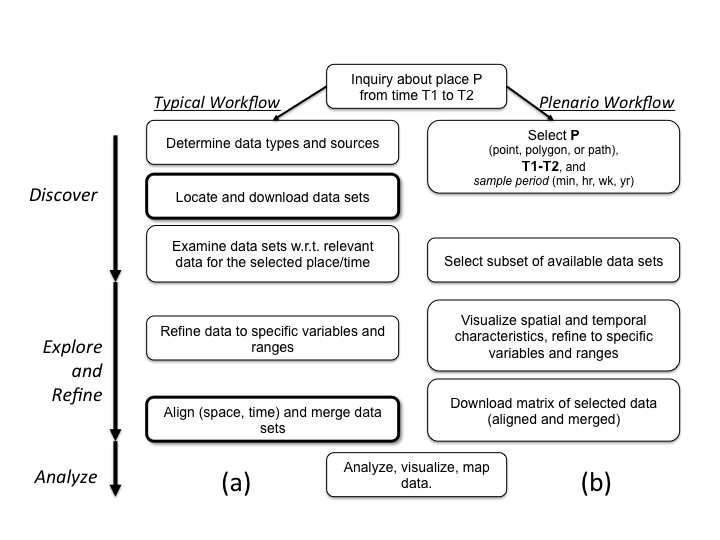
\includegraphics[scale=.5]{plenario_workflow.png}
\end{figure}

The Plenario project began with a hypothesis that for open data is to have truly transformative impact, it must be accessible to non-data scientists, by individuals without a priori familiarity with the growing collection of open data portals (or their user interfaces), and it must be possible to explore the data without first investing weeks or months in data preparation. Plenario is a prototype platform developed to test this hypothesis by bringing many open data sets together, integrating them, and presenting a map-based interface for users to discover data sets relevant to a particular place over a period of time, and to examine the potential for interdependencies among those data sets.

\subsection{Plenario: An Overview}
Plenario exploits the fact that the vast majority of open data portals are implemented using one of two platforms, each with an API for accessing and downloading data---Socrata Open Data API (SODA) \cite{socrata} and Comprehensive Knowledge Archive Network (CKAN) \cite{ckan}. Each platform offers various internal search capabilities, visualization tools, and APIs for external application development. Yet at present there is no federation of these platforms or global search capabilities. In part the lack of search capabilities reflects the fact that the data is highly diverse, from text to spreadsheets to shapefiles, and it is not clear how one might search such a collection of sources---keyword? Full text? Based on interactions with the US-RCN community and the experience with WindyGrid in the City of Chicago, Plenario is designed to support place and time inquiries, and consequently uses a map interface with time specifications to implement search. This user interface replaces the first two steps in typical workflows---the ``Discover'' phase shown in Figure \ref{fig:plenario-workflow}.

Beyond the need for search, open data sources are diverse with respect to their spatial and temporal organization, resolution, units of measure, and other factors. Plenario imports data sets and integrates them into a single geospatial database, performing the alignment and merger of the data sets, eliminating the need for the user to do so, as shown in the ``Explore and Refine'' phase of Figure \ref{fig:plenario-workflow}. Moreover, the Plenario workflow does not rely on the knowledge of the user to determine where relevant data might exist. In cases where the use may be aware of data that is not within Plenario, a request for data import is provided through a web form.

Figure \ref{fig:plenario-workflow}(b) illustrates the Plenario workflow, with its new open data discovery capability and automation of several of the most costly steps in the data analysis workflow---notably the ``Locate and download'' and ``Align and Merge'' steps in Figure \ref{fig:plenario-workflow}(a). Instead of searching for and combing through a multitude of potential open data sources and datasets to find data of interest for a particular location, the user specifies geographical boundaries and instantly receives all of the data available for that location (Figure \ref{fig:plenario-search-example}). The labor-intensive work of combining and aligning the various spatial and temporal attributes of data sets is already done as part of the data import functions of Plenario, significantly shortening the path from question to discovery.

Plenario also provides basic data visualization, mapping, and time series creation to give users a snapshot of data before they decide to download it (Figure \ref{fig:plenario-dataset-vew}). When data sets are listed in response to a user query, each includes not only basic information and links to provenance and meta data, but a simple time series graph that provides the user with an indication as to the overall signal of the data set, for instance whether it might provide relevant information for the particular temporal query. Data sets can be selected for a map-based view showing spatial density of the data, and the user can modify the aggregation density from 100 meters to 1 kilometer. Finally, the user can refine the view of a selected data set by specifying fields and values or ranges of interest. All of these tools enable the user to examine each data set to determine its relevance to the research questions before exporting the integrated data sets of interest.

Furthermore, the platform helps avoid duplication of effort by providing a space for users to collaborate on cleaning data and exploring datasets in more sophisticated ways. Every dataset only needs to be imported once but can be used by all (or all authorized users if the data set is not open); similarly, all results of data cleaning are available for all users.

\section{Plenario Architecture and Implementation}
The Plenario software platform is open source and available at GitHub \cite{plenario-github}. It is implemented using Amazon Web Services commercial cloud services. This facilitates replication in several important ways. First, governments and other organizations can readily create an instance of Plenario for their use, potentially including both open and internal data. Second, organizations can provide open data for integration into an existing Plenario instance, such as the one operated by the University of Chicago at http://plenar.io. They can then use Plenario's analysis tools and API to power their own applications. The architecture allows data providers to choose which datasets are available to the public and which should remain ``closed,'' available only for internal use for authorized users. The San Francisco Plenario instance, detailed below, is being used to explore functions for aggregating sensitive data prior to presenting to the end user. 

Here we describe the Plenario architecture, comprising (a) data import via an automated Extract-Transform-Load (ETL) builder, (b) integration using a geospatial database, and (c) special cases for common data sets such as weather and census data. In brief, an automated extract-transform-load (ETL) builder imports each dataset and inserts the table into a PostgreSQL database. The ETL builder includes a specification for update frequency, so that Plenario updates the dataset at the same frequency as the source dataset is updated. Every row in the dataset is represented by a pointer in a single ``Master Table'' so that all data is indexed on the same spatial and temporal indices (Figure \ref{fig:flowchart}). The platform then joins each observation to a set of commonly used data sets including sensor and place-based data and exposes the dataset in the relevant API endpoints and through the web portal view.

\subsection[data-import]{Data Import: \textbf{Automated ETL Builder}}
A dataset is submitted to Plenario as a URL linking to a publicly available table in CSV format, which includes any datasets on a Socrata or CKAN platform or self-hosted by the user. Plenario's automated ETL builder scans the dataset, infers field types, and checks for common issues of data integrity. As Plenario currently focuses on spatio-temporal datasets, the user is then asked to identify which fields correspond to the spatial field(s), temporal field, and unique ID, and how frequently the dataset updates\footnote{Future improvements to Plenario will remove one, two, or all three of these requirements: see discussion in Section \ref{sec:challenges}}. The user can also add information regarding the dataset's provenance, description, and license if these are not automatically populated (as they are with Socrata datasets). 

Following a basic check for URL stability and malware, an ETL worker process begins importing a local copy of the dataset as a new table in the PostgreSQL database. After import, Plenario inserts a row into the Master Table for every row in the new dataset, containing the dataset ID, the row ID (unique ID), and the spatial and temporal fields. The dataset is then made available via a RESTful API with endpoints for raw data, data aggregation by time and space, metadata, and weather-specific data (weather is one of several special case base data sets discussed in Section \ref{sec:commonly-used-datasets}). Tasks are automatically scheduled to update the dataset according to the refresh frequency of the source dataset, using the unique ID to avoid re-populating the entire table. Datasets can be imported and updated simultaneously using multiple ETL workers.

\begin{figure}
	\centering
	\label{fig:flowchart}
	\caption{The path from identification of an appropriate dataset to making it available in the Plenario API. This process takes less than 24 hours for all but the largest datasets; we aim to improve this efficiency much further.}
	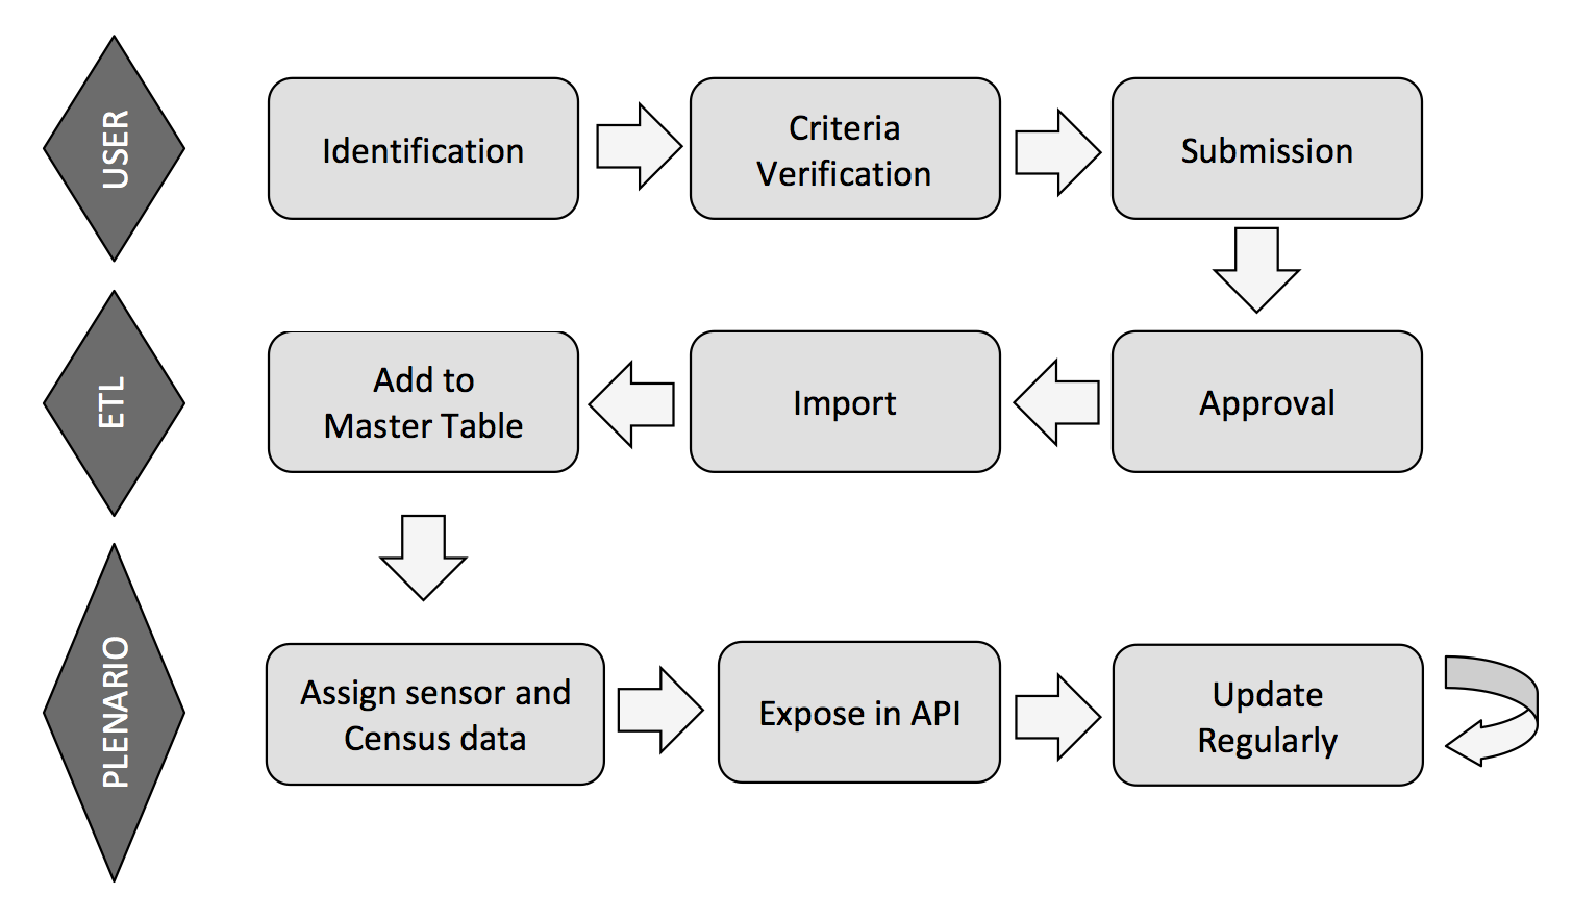
\includegraphics[scale=.45]{flowchart.pdf}
\end{figure}

\begin{figure}
	\centering
	\label{fig:plenario-search-example}
	\caption{An example search using the portal interface (showing only the first 4 of 18 data sources found for this area at the specified time window. Note the time series (weekly aggregation specified) graphs providing the user with an indication of temporal dynamics of all data sets found.\vspace{.4cm}}
	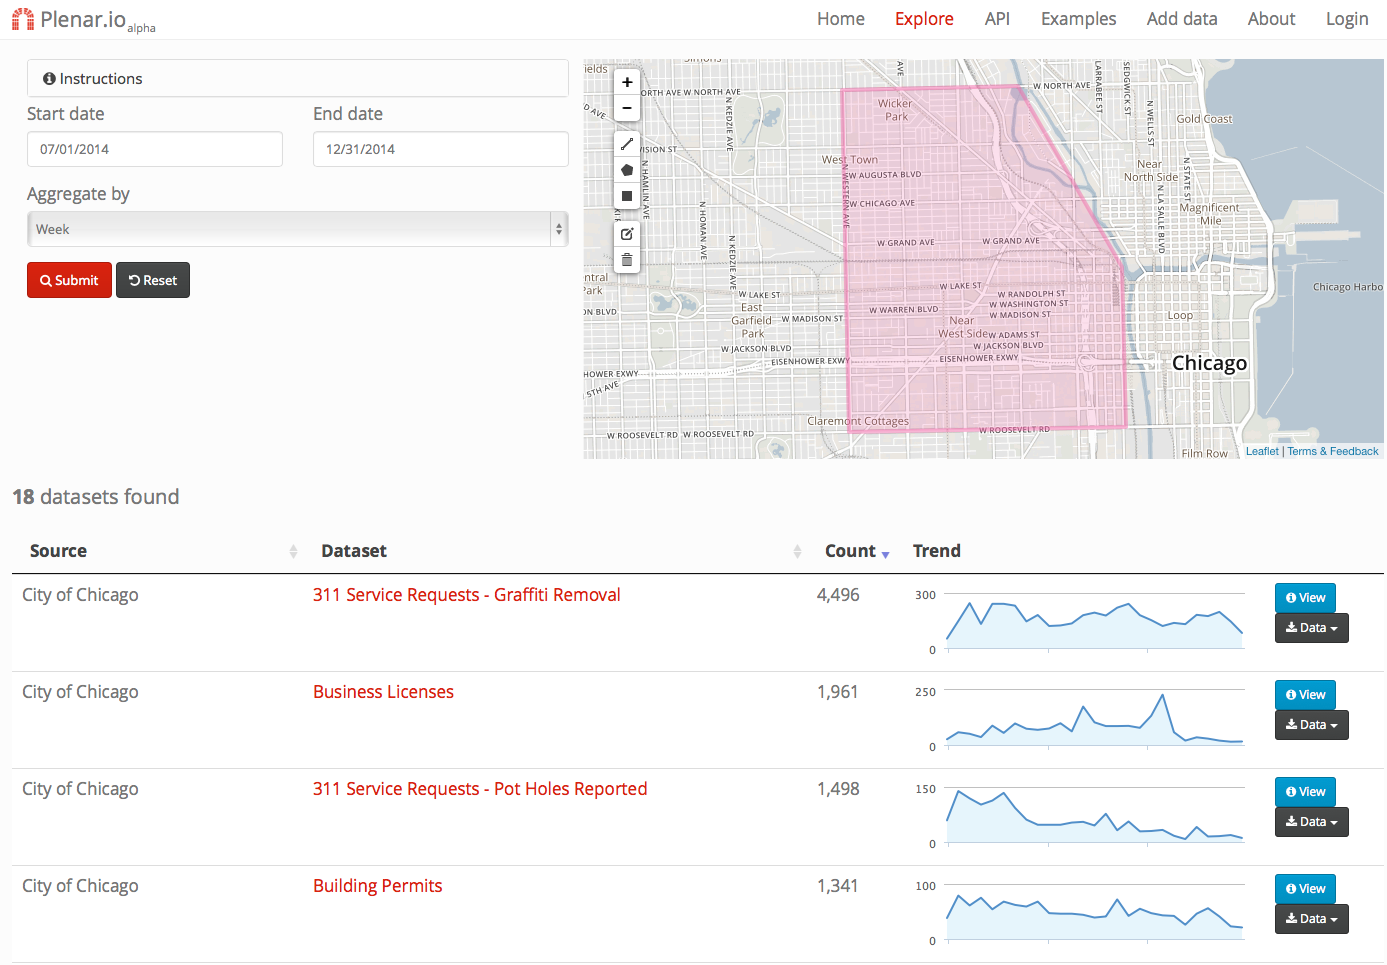
\includegraphics[scale=.25]{plenario_search_example.png}
\end{figure}

\begin{figure}
	\centering
	\label{fig:plenario-dataset-vew}
	\caption{Plenario data set view. Selected from the first results screen, this view allows the user to view the spatial distribution of a given data set and provides links to the data and associated metadata. This screen also allows the user to change the temporal and spatial resolution of the query and to refine the data set by selecting and specifying values or ranges for individual record values.\vspace{.4cm}}
	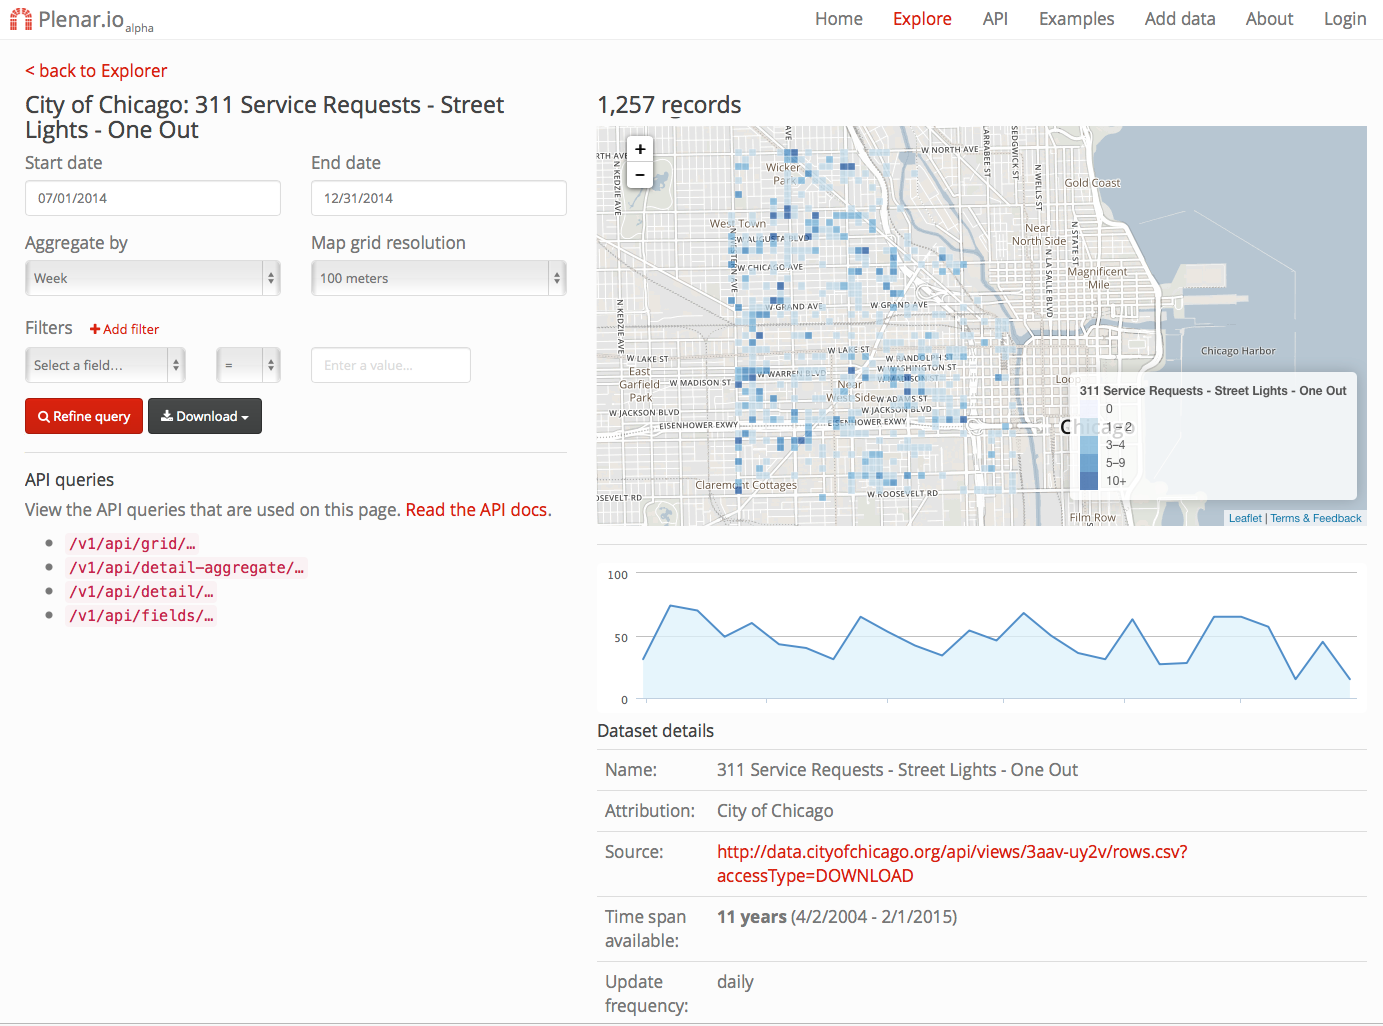
\includegraphics[scale=.25]{plenario_dataset_view.png}
\end{figure}

\subsection{\textbf{Core Database: Single Spatio-Temporal Index and PostgreSQL Schema}}\label{sec:core-database}
Plenario achieves the workflow optimizations discussed in Section \ref{sec:context-objective} and illustrated in Figure \ref{fig:plenario-workflow} by organizing all records using common spatial and temporal indices in the Master Table (Figure \ref{fig:db-schema}). This method has several important implications. 

First, it automatically organizes data in an intuitive and coherent way that is easily manipulated by the user. In addition to the API endpoints, Plenario includes a portal interface (Figure \ref{fig:plenario-search-example}) through which users can draw polygons or paths on a map and select start and end dates to search for relevant datasets. 

Second, it organizes this data without relying upon user knowledge of the existence of the data or its sources. Any point or polygon, and any time period, could be associated with data from multiple datasets, from multiple government agencies or organizations, and this data is retrieved without the need to specify the data source. That is, a query for data points from Midtown Manhattan during June 2013 would return data from the City of New York, New York State, the federal government, and numerous local or national organizations and surveys, including sources of which the user was unaware. 

The third implication is that data for any arbitrary geography can be readily organized as a time series containing counts (or other variables) of observations in each contained dataset. Plenario enables one-click download of such time series matrices, instant snapshots of a geography over time, with any temporal resolution from hours to decades. In this way, it removes the tedious work of data compilation and aggregation along identical temporal and spatial units and allows users to instantly begin simple analyses.

\begin{figure}
	\centering
	\label{fig:db-schema}
	\caption{PostgreSQL Schema, showing how a sample dataset (Chicago crimes) feeds into the Master Table, which in turn links to spatial data like Census blocks and sensor data like weather observations through the \texttt{census\_block\_id} and \texttt{weather\_observation\_id} fields. There is one row in the Master Table for every row in a source dataset like Crimes, but a many-to-many relationship exists between the Master Table and Census blocks or weather observations. Note that the \texttt{Weather\_Observations\_Hourly} table (which contains no spatial information) is filtered through the \texttt{Weather\_Stations} table (which contains no temporal information). \vspace{.4cm}}
	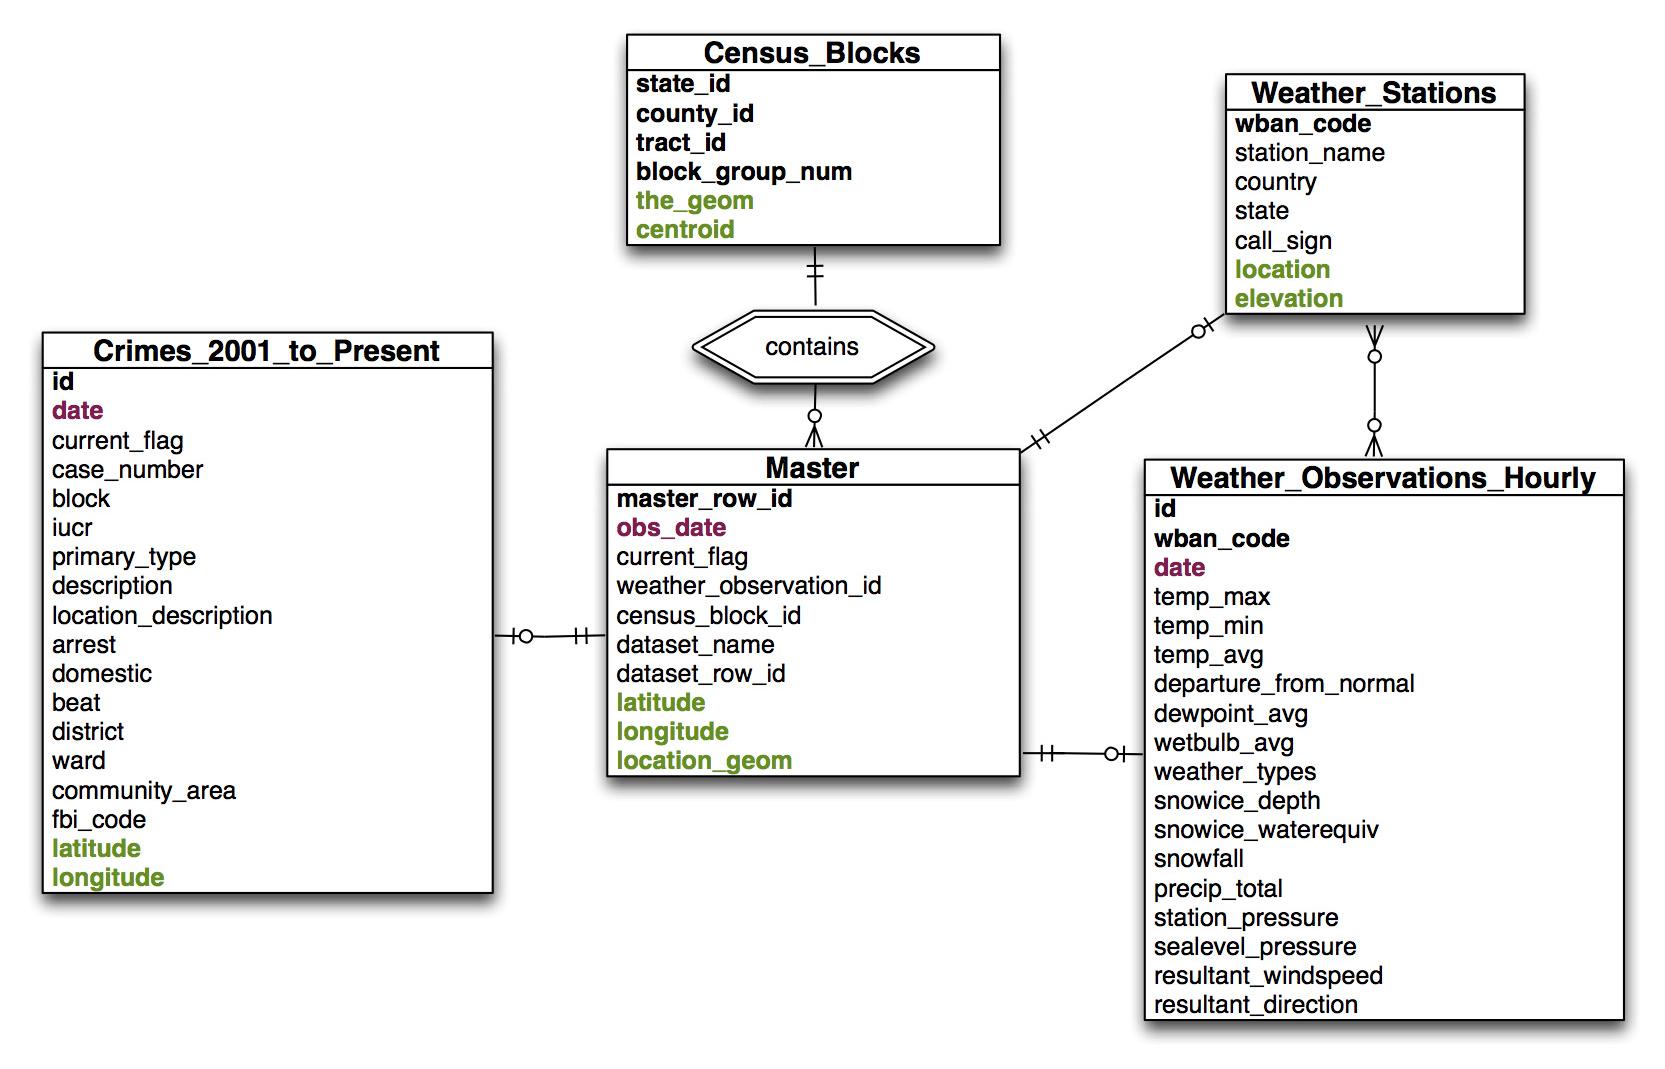
\includegraphics[scale=.45]{db_schema.pdf}
\end{figure}

\subsection{\textbf{Special Cases: Commonly Used Data Sets}}\label{sec:commonly-used-datasets}
Plenario was optimized to support not only particular data sets related to a specific topic but to enable investigations in context of widely used data sources such as weather and location shapefiles, and aggregated census information. Once a dataset is imported and inserted into the Master Table, Plenario enriches it with other data relevant to the same geography, including sensor and location-specific data. Below we discuss \textit{sensor data} (time series such as weather) and \textit{local data} (relatively static data about the geography), which are also shown in Figure \ref{fig:db-schema}.

\textit{Sensor data}, which records one or more variables at regular intervals in fixed locations, usually along a network with high coverage (such as weather stations), is important both for tracking environmental variables over time and for enhancing human-generated data (such as noise complaints) with objective recordings from the same time and location (such as noise levels). 

Weather data in particular is important to many questions about place, ranging from healthcare studies to traffic or flooding analysis. Hourly and daily weather data from NOAA is thus ``baked into'' the Master Table scheme, providing an initial example of how sensor data adds to the open data landscape. After loading in all hourly and daily weather data across the United States since 2011, Plenario assigns to every record in the Master Table the weather station that is closest to it. In response to any query requesting weather information about that record, Plenario retrieves the observation from the weather station nearest the location of the record and for the time closest to the record's timestamp. The process is efficient because all weather data is stored in only one place, and because the closest weather stations are pre-calculated when a dataset is imported. 

Further plans for sensor data include incorporating data from the Array of Things \cite{moser_2015} project in Chicago, which will report measures such as air pollution and noise at a much higher resolution both temporally (every 30-60 seconds) and spatially (the sensors will be deployed throughout Chicago with densities ranging from one per square block to one per square kilometer). This data source will further illustrate the value of sensor data to municipal open datasets, enabling investigations such as the spatial and temporal characteristics of air quality in context of vehicle flow and weather, or the interrelationships between hyperlocal weather and crime. 

\textit{Local data} refers to data aggregated at a regional (not individual) level containing variables that are relatively static over time, such as demographic data and local economic data. The University of Chicago implementation of Plenario incorporates a prototypical example of local data, which is data from the United States Census: every row in the Master Table is coded with its FIPS Census block ID, which allows for easy enhancement with open data from other sources tied to that Census block, Census tract, county, state, etc., all of which can be determined from the Census block ID. 

\subsection{Components and AWS Implementation}
Plenario is built entirely from open source tools and is released under the MIT license. All code is in a GitHub repository \cite{plenario-github}, making the platform easy to fork and clone. Source datasets remain under their original license; most are released under the MIT license or are unlicensed. 

The platform is built as a PostgreSQL and PostGIS geospatial relational database. SQL Alchemy \cite{sqlalchemy} is used as the object relational mapper with the GeoAlchemy 2 extension. The web application with API was developed using Flask \cite{flask}, with mapping capabilities provided by Leaflet \cite{leaflet} and Open Street Map \cite{openstreetmap}. The ETL process uses Celery \cite{celery} for logging, and Redis \cite{redis} is available for caching support when high loads are anticipated. 

Plenario is hosted by Amazon Web Services (AWS) on their Elastic Cloud Compute (EC2) infrastructure. Four virtual servers are utilized within a Virtual Private Cloud (VPC): one web server, one database server, one ETL worker server and one gateway server. Due to its elastic nature, the EC2 server resources can be upgraded in real time as traffic load and data footprint increase. For larger deployments, the database server can be sharded and replicated for more capacity using the Amazon Relational Database Service (RDS). Amazon Machine Images (AMI) can be utilized to take a snapshot of each server configuration for easy re-deployability.

For data integrity and redundancy, every raw dataset processed by the Plenario ETL worker is saved as a snapshot and stored on Amazon's Simple Storage Service (S3). This allows for data integrity checks, ETL fault tolerance and history tracking on every dataset Plenario ingests.

There are several ways for the community to use Plenario: a user can fork the GitHub code to develop a separate project, copy the entire project via a machine image on AWS, or feed data into the web portal supported by the University of Chicago at http://plenar.io. All of these modalities of use have been seen since Plenario's alpha launch in September 2014, including a repurposing of the core API to power the City of San Francisco's Sustainable Systems Framework initiative as detailed below. 

The web portal interface described above is in fact an application that accesses Plenario via the API. This modular approach enables other front-end frameworks to be built to use the API, from custom mobile and web applications (of which http://plenar.io is an example) to a complex analytics system such as WindyGrid, which uses commercial mapping and user interface software such as from ESRI.

\section{Evaluating Plenario's Architecture}
% Characteristics of the database
The key architectural feature of the Plenario system is its spatio-temporal database, which is hosted on the cloud. A RESTful API is used to upload new datasets into the hosted system, and to query datasets for discovery and exploration. The system, given its need to support open-data of all, sets no limit on the amount of data a user can upload, both in terms of  the number of uploads and the size of the upload. The open upload feature raises a scalability concern, especially when performing exploratory spatial querying---a feature which can itself be I/O-intensive. A concern complementary to scalability but related is the cost of hosting an open-data service such as Plenario on the cloud. Given the volume of anticipated data, hosting Plenario on high-end instances seems natural but if most uploads are small and queries retrieve small spatial regions then high-end instances do not provide sufficient cost-benefit advantage. 

To evaluate our choices, we performed a through performance evaluation and determine the right choice of the database that can support efficient and concurrent uploads and querying, and to determine which type of cloud instance provides the best cost-benefit ratio. To conduct the experiments, we developed a benchmark based on available Plenario queries and logs. We evaluated the benchmark workload with relational, NoSQL and array databases to determined which database exhibits highest performance for concurrent uploads and query. Finally, we instantiated Plenario's relational database on different cloud-instances to determine the best cost-benefit ratio in terms of transactions per second per dollar spent.

% Benchmark specification
\subsection{The Plenario Benchmark}
We developed a benchmark specific to Plenario becuase unlike other geospatial benchmarks, Plenario has no separate database instantiation and query generation phase; database tables and queries are determined by an incoming user-workload leading to an openly-writable spatial storage system. To simulate the discovery and exploration phases in Plenario, we simulated a closed loop Markov-chain synthetic workload generator in Python. The  Markov-chain consists of two different states, ``add\_data'' and ``query", in which the ``query phase'' consists of five different states, including ``initial\_query'', ``expand\_time'', ``narrow\_time'', ``expand\_geography'' and ``narrow\_geography''.
The current state gets updated after each query and the system chooses between query with probbability 0.85 and upload with probability 0.15. Within the query phase expansion and reduction of spatial attributes occurs with equal probability, and spatial attributes are chosen over time attributes by 0.6 to 0.4. These probabilities are chosen based on user query logs and estimated patterns. 

%Constructed a transition matrix with 6 different states: %"add\_data", "initial_query", "expand_time", "narrow_time", "expand_geog" and "narrow_geog". The latter states "expand_time", "narrow_time", "expand_geog" "narrow_geog" and �stop� can only take place if the current state is �initial_query�. 
%The current state gets updated after each query. The probability is set based on an estimate on the user query patterns, and should ideally be learned from actual user query logs

\subsection{Evaluation}
% Evaluation


\section{Plenario Use Cases and Early Lessons Learned}
We have discussed a number of advantages the Plenario project was designed to provide for researchers, government employees, developers, journalists, and citizen users. Here we discuss several specific use cases where Plenario is providing support for social and economic science research (The Chicago Plenario instance) and for community engagement on urban sustainability, resilience, and livability goals (The San Francisco Plenario instance). 

\subsection{\textbf{Supporting Research: The Chicago Instance}}\label{chicago-instance}
The Chicago instance of Plenario, active at http://plenar.io, has been implemented with data from multiple cities, and with a focus in particular on Chicago, to support research\textit{ }into urban science and computational approaches to public policy, identified through the US-RCN, by supporting rapid data discovery, helping researchers, journalists, and residents identify datasets that interest them regardless of the original source. For example, Goldstein leads a team investigating the interrelationship between local weather and violent crime, which involves all of the base sensor and local data described in Section \ref{sec:commonly-used-datasets} as well as urban crime data, 311 service call data, and other data sets. Without Plenario, this research would begin with an attempt to find data of interest from many independent sources, many of which the user might not know exist. For Chicago these include open data portals operated by the City of Chicago, Cook County, the State of Illinois, the federal government, and data from hundreds of separate government departments such as the Illinois Department of Transportation or the Chicago Department of Public Health. In addition to these sources, relevant data has been imported into http://plenar.io from the National Oceanic and Atmospheric Administration (NOAA) and the U.S. Census Bureau. 

As the Chicago instance has grown from dozens of data sets to over 150, the quality of source data has been more readily exposed due to the automatic data set summaries produced in response to user searches. A single error in the date field, for instance, results in a summary that suggests Plenario contains data from prehistoric times, or far into the future. A set of consistency checks to flag obvious errors of this kind (such as impossible dates) is a sensible approach, but all errors are not readily flagged by algorithms. The very nature of data is that errors and holes are inevitable, and thus it will be important to not only work with data providers to fix obvious errors but to provide Plenario users with mechanisms to discover and flag errors. 

With goals to expand the Chicago instance to thousands of data sets, the team is also beginning to analyze the scalability of the Master Table approach and of the specific database implementation.

\subsection{\textbf{Enabling Community-Driven Urban Sustainability, Resilience, and Livability: The San Francisco Instance}}\label{san-francisco-instance}
The platform is also deployed experimentally as part of the City of San Francisco's Sustainable Development initiative \cite{sf-sustainable-systems}. This project has led to Plenario enhancements necessary to support additional data types and the use of Plenario as a community ``dashboard''---where the visual interface is the primary use, in contrast to the Chicago deployment, which emphasizes the need to refine and export data for advanced data analytics. In several cases, notably the support for adding geographical information in the form of ESRI shapefiles to the database, the San Francisco implementation has driven key enhancements to the core Plenario code base. In other cases there are customizations that will be incorporated after evaluation in the San Francisco instance.

The San Francisco Plenario instance contains datasets pertaining to a wide variety of sustainability indices, ranging from community structures accessibility, to green space and canopy cover, to water and energy consumption. Having the ability to instantly access datasets of this kind by spatial-temporal queries greatly empowers institutions and communities to assess the status quo and plan future efforts in sustainable development. In particular, the framework is to be used in the sustainable development of the South of Market (SoMa) ecodistrict.

The data needed for this type of system is very heterogeneous, both in content and form. For example, quantifying access to green spaces---the vicinity of parkland to residents---requires analysis of geographic information regarding the location and shape of the park, which is not simply a point in space. Similarly, a community center is an entity that exists over a certain time span, in contrast to much place-based urban data such as crime or inspections, which are ``events'' that occur at a specific instant. To incorporate these and other types of data, Plenario's database schema was extended and more ETL functions were added. Moreover, new types of queries were developed and implemented efficiently, aimed at questions of the type ``What is the average distance for residents of a given area to the closest farmer's market, at any point in time and in a given range?''

The San Francisco Plenario instance is also exploring approaches to support a mix of open and sensitive data. As with the Census data in the Chicago instance, some of the data in San Francisco is not public and is thus carefully aggregated to protect privacy. One algorithm that is commonly used for utilities datasets is the ``15/15 rule,'' which requires that no aggregation sample may contain less than 15 data points, and any point in any aggregation sample cannot represent more than 15\% of the measure for that sample\footnote{The ``15/15 Rule'' was adopted by the California Public Utilities Commission in Decision D.97-10-031.}. The methodology being explored in the San Francisco project is for the ``providers'' of the Plenario instance to securely host the raw data, executing the query- and data-specific privacy-preserving aggregations as a function of the particular search, view, and/or data export process.




\section{Lessons, Challenges, and Opportunities}\label{sec:challenges}
With the two large-scale Plenario instances described above, we have identified a number of challenge areas that will be essential to address in order to move Plenario from an alpha platform to a fully supported and sustainable resource. We group these as issues related to data, scaling, and architecture. 

\subsection{\textbf{Data Issues}}
Data is often collected in very different ways across jurisdictions, because every local government has slightly different goals in mind. Even datasets with very similar purposes, such as 311 service requests or food safety inspection reports, can rarely be merged across jurisdictions, effectively limiting research to a focus on one particular city rather than incorporating and studying multiple cities at once. These barriers can exist at the metadata level (different variables recorded), in the resolution of the data (spatial and temporal), and even at the level of individual data points and fields (semantics and ontology). For example, a crime classified as ``assault'' in New York City crime data would be classified as a ``battery'' in crime data from Chicago, which may mislead a researcher attempting to compare violent crime in the two cities or compile a large dataset of crime in the United States. 

We have also encountered the common challenge of poor data quality and documentation. Because all data in Plenario ultimately refers to a source dataset hosted by a municipality, the remedy is limited to either cleaning the data upon insertion into Plenario or providing feedback to the data providers. Data cleaning at insertion would accelerate cleaning in comparison to relying on data providers, but would also require that the platform understand in each case what is ``correct.'' Ultimately this balance might be encoded into the ETL process in similar fashion to the update frequency. Finally, the lack of unique IDs on many datasets also means that updating datasets requires a full refresh of the entire dataset, which increases load but more importantly introduces data consistency issues that will impact the applications using the datasets, particularly those aimed at real-time capabilities. 

\subsection{\textbf{Scaling Issues}}
Plenario was designed with consideration regarding scale, given the enormity of the open data landscape and the rapid pace with which open datasets are being released. Nevertheless, as the experiments show the Master Table approach introduces scaling challenges, particularly as the table grows to billions of rows. The team has explored a variety of approaches including partitioning the table along the temporal index, with mixed results. In particular, the number of NOAA's hourly observations for all 2,200+ weather stations since 1997 in the United States was deemed too large to import in its entirety, while maintaining a reliably responsive API. To work around this limitation, only observations from weather stations within a certain radius of each dataset's bounding box were added.

The sensor data also contributes to scaling challenges. Though the closest weather station to every record is identified upon insertion into the Master Table, the platform executes the join at the time of request rather than as part of the insertion process. This has significant impact on query performance but the alternative would exacerbate scaling issues with the Master Table by making it extremely wide. Furthermore, sensor data needs to be spatially smoothed to avoid sharp boundaries in the data such as when two neighboring weather stations record significantly different values for a given variable. To reduce computational load, sensor data is organized spatially using a Voronoi diagram \cite{voronoi_1908} without spatial smoothing.

\subsection{\textbf{Architecture and Data Semantics Issues}}
Plenario's original purpose as a platform for spatio-temporal data discovery and exploration brings into question what variables count as ``space'' and ``time''. For example, should 311 data reflect the location of the caller or the location of the problem reported? How should the location of non-spatial crimes, like fraud or online crimes, be reported? And how should Plenario represent records missing a spatial or temporal value? How, too, could unstructured data be supported in Plenario - especially when the location and datestamp of such data are uncertain?

We have also encountered challenges with respect to how to treat data that lacks resolution in spatial and temporal data. For instance, how do we present city budget data that covers an entire city for the period of one year-{}-and make this data discoverable in typical user searches? Should a query across multiple years return multiple city budgets, ones wholly contained in the temporal arguments, or none at all? How should shapes like parks, streets, and parcel lots be dated? Some of these challenges are being highlighted in the San Francisco Plenario instance, as discussed earlier.

Ultimately these challenges suggest exploration into the optimal approach to support the integration of spatial/temporal data with data that is primarily ``entity'' based. In some cases, such as with census data, spatial and temporal mapping can be done in concert with data aggregation as is necessary for privacy protection. In other cases, particularly with organizations whose data includes internal private data about businesses and individuals, such mapping is less straightforward. Plenario currently supports questions such as ``where were the automobile accidents in mid-town Manhattan during heavy rainstorms in 2014'' but is not organized in order to refine this query to show only those accidents involving cars greater than 10 years old, or male drivers aged 18-24.

Finally, Plenario is currently designed as a portal for open data, which is only a subset of data useful for urban science and research, for policy development, or for many areas of improved urban operations. There are known solutions to challenges to multiple levels of authorization, and it will be important to integrate these into the platform. The San Francisco Plenario instance supports sensitive data by aggregating at the time of query, presenting the aggregated data to the end user. The Chicago Plenario instance uses pre-aggregated census data, eliminating the need to aggregate at query time. While this improves query performance and reduces the sensitivity of the data stored in Plenario, it also requires that the aggregation algorithm is defined a priori, where different aggregation schemes may be more or less optimal for different types of inquiry.

\section{Conclusions and a Plenario Roadmap}
The Plenario team has begun to develop a 12-18 month roadmap based on input from early users. A rigorous set of performance scaling tests is being developed to explore the architecture issues noted above, and this will involve revisiting decisions ranging from underlying database to the design of the Master Table. Several features requested by researchers are under consideration for this roadmap, including automated time series analysis to identify correlations between datasets: for instance, drawing attention to subsets of 311 data which are lagged by violent crime in various neighborhoods of a city. 

Of particular interest to many place-based investigations is the identification of urban ``areas'' that function as units. Traditional boundaries such as neighborhoods or districts often do not reflect the underlying social or economic structure, in part because many such boundaries were drawn generations in the past and/or through political processes. The rapidly expanding variety of data being integrated into Plenario is resulting in increased opportunity to understand what differentiates one neighborhood from another and to use spatial units defined by current data, not solely by a 20\textsuperscript{th} century surveyor's pen. Concurrently, support for place-based research will require more powerful tools for specifying spatial aggregation of data (where Plenario has already provided flexibility in temporal aggregation), necessary to address the Modifiable Area Unit Problem \cite{wong_2009}, or the fact that the results of spatial analysis are often highly dependent on the spatial units used.

Today's open data landscape largely resembles the Internet of the 1980s when data was shared through anonymous file transfer servers, which were useful only to those with inside knowledge of their locations and contents. The advent of HTTP and web browsers led to today's powerful search and integration capabilities (including those Plenario uses to import data!), and an underlying objective of the Plenario project is to contribute to these benefits extending to open data.

The first step toward this vision has been to implement the Plenario platform as a means to reduce or eliminate many of the challenges of working with open data, beginning with discovery, exploration, and integration across many data sources. Addressing these challenges provides increased incentives for governments to release data, reducing the need to develop their own custom data portals and providing the basic tools to start extracting insight and return on investment from their data. By building and encouraging a collaborative open data ecosystem at every stage, from identifying datasets to building third-party tools, Plenario helps push the full potential of this movement closer to realization. 

\section*{Acknowledgments}
The Plenario project is funded by the John D. and Catherine T. MacArthur Foundation and the National Science Foundation via an NSF Early-Concept Grant for Exploratory Research (EAGER) for software development (award number 1348865), while the interaction capabilities were driven by the Urban Sciences Research Coordination Network, created with an NSF Building Community and Capacity for Data-Intensive Research in the Social, Behavioral, and Economic Sciences and in Education and Human Resources (BCC-SBE/EHR) award.




\begin{thebibliography}{1}

\bibitem{maksimovic_2011}
Maksimovic, M.D.; Veljkovic, N.Z.; Stoimenov, L.V., ``Platforms for open government data,'' Telecommunications Forum (TELFOR), 2011 19th, vol., no., pp.1234,1237, 22-24 Nov. 2011. doi: 10.1109/TELFOR.2011.6143774

\bibitem{windygrid}
``Chicago's WindyGrid: Taking Situational Awareness to a New Level.'' \url{http://datasmart.ash.harvard.edu/news/article/chicagos-windygrid-taking-situational-awareness-to-a-new-level-259} [Accessed July 7, 2015]

\bibitem{urbanccd}
The Urban Center for Computation and Data, at the Computation Institute of the University of Chicago and Argonne National laboratory. \url{http://www.urbanccd.org} [Accessed July 7, 2015]

\bibitem{us-rcn}
NSF 1244749, ``BCC-SBE: An Urban Sciences Research Coordination Network for Data-Driven Urban Design and Analysis. \ PI Catlett, C., University of Chicago. 2012-2015.

\bibitem{socrata}
\url{http://www.socrata.com/} [Accessed July 7, 2015]

\bibitem{ckan}
\url{http://ckan.org/} [Accessed July 7, 2015]

\bibitem{plenario-github}
\url{https://github.com/UrbanCCD-UChicago/plenario} [Accessed July 7, 2015]

\bibitem{moser_2015}
Moser, W, ``What Chicago's `Array of Things' Will Actually Do,'' Chicago Magazine, January 27, 2014. See also \url{http://ArrayofThings.github.io} [Accessed July 7, 2015]

\bibitem{sqlalchemy}
\url{http://www.sqlalchemy.org/} [Accessed July 7, 2015]

\bibitem{flask}
\url{http://flask.pocoo.org/} [Accessed July 7, 2015]

\bibitem{leaflet}
\url{http://leafletjs.com/} [Accessed July 7, 2015]

\bibitem{openstreetmap}
\url{http://www.openstreetmap.org/about} [Accessed July 7, 2015]

\bibitem{celery}
\url{http://www.celeryproject.org/} [Accessed July 7, 2015]

\bibitem{redis}
\url{http://redis.io/} [Accessed July 7, 2015]

\bibitem{sf-sustainable-systems}
``The Sustainable Development Program.'' \url{http://www.sf-planning.org/index.aspx?page=3051} [Accessed July 7, 2015]

\bibitem{voronoi_1908}
Voronoi, G., Nouvelles applications des param\'etres continus \'a la th\'eorie des formes quadratiques. Deuxi\`eme m\'emoiure: recherches sur les parall\`eloedes primitifs, J. reine angew. Math. 134, 198-287 (1908)

\bibitem{wong_2009}
Wong, D., ``The modifiable areal unit problem (MAUP)'', In Fotheringham, A Stewart; Rogerson, Peter. \textit{The SAGE handbook of spatial analysis}. pp.~105--124 (2009)

\end{thebibliography}







\end{document}